\documentclass[11pt,a4paper]{article}
% Shared styling for the WaveKitchen documentation PDFs.
\usepackage[T1]{fontenc}
\usepackage{lmodern}
\usepackage[utf8]{inputenc}
\usepackage[margin=2.2cm,headheight=14pt]{geometry}
\usepackage{amsmath,amssymb}
\usepackage{xcolor}
\usepackage{booktabs,longtable,tabularx,array}
\usepackage{enumitem}
\usepackage{fancyhdr}
\usepackage{titlesec}
\usepackage[most]{tcolorbox}
\usepackage{tikz}
\usetikzlibrary{arrows.meta,positioning,shapes.geometric,calc,fit}
\usepackage{microtype}
\usepackage[hidelinks]{hyperref}
\urlstyle{tt}

\definecolor{wkorange}{HTML}{E0661E}
\definecolor{wkteal}{HTML}{0E8A8A}
\definecolor{wkink}{HTML}{1F2937}
\definecolor{wkgrey}{HTML}{6B7280}
\definecolor{wkred}{HTML}{B91C1C}
\definecolor{wkgreen}{HTML}{15803D}
\definecolor{wkpaper}{HTML}{FFF8EF}

\hypersetup{colorlinks=true,linkcolor=wkteal,urlcolor=wkteal,citecolor=wkteal}

\titleformat{\section}{\Large\bfseries\color{wkorange}}{\thesection}{0.8em}{}
\titleformat{\subsection}{\large\bfseries\color{wkink}}{\thesubsection}{0.7em}{}
\titleformat{\subsubsection}{\normalsize\bfseries\color{wkteal}}{\thesubsubsection}{0.6em}{}

\setlist{itemsep=2pt,topsep=4pt}
\setlength{\parskip}{4pt}
\setlength{\parindent}{0pt}
% long unbreakable code names: stretch spaces rather than overflow the margin
\setlength{\emergencystretch}{3em}
\renewcommand{\arraystretch}{1.25}
% ragged-right paragraph column (no stretched inter-word spaces in narrow cells)
\newcolumntype{P}[1]{>{\raggedright\arraybackslash}p{#1}}

% file paths (break at slashes) and code identifiers (underscore-safe)
\newcommand{\file}[1]{\nolinkurl{#1}}
\DeclareRobustCommand{\fn}[1]{\texttt{\detokenize{#1}}}
% plain text for PDF bookmarks when these appear in headings
\pdfstringdefDisableCommands{\def\file#1{#1}\def\fn#1{\detokenize{#1}}}

\newtcolorbox{conceptbox}[1][]{colback=wkteal!6,colframe=wkteal,fonttitle=\bfseries,
  title={Signals \& Systems concept#1},breakable,left=6pt,right=6pt,top=4pt,bottom=4pt}
\newtcolorbox{impactbox}[1][]{colback=wkorange!6,colframe=wkorange,fonttitle=\bfseries,
  title={Why it is here \& its impact#1},breakable,left=6pt,right=6pt,top=4pt,bottom=4pt}
\newtcolorbox{filesbox}{colback=wkink!4,colframe=wkink!70,fonttitle=\bfseries,
  title={Files involved},breakable,left=6pt,right=6pt,top=4pt,bottom=4pt,before upper=\raggedright}
\newtcolorbox{flagbox}[1][]{colback=wkred!5,colframe=wkred,fonttitle=\bfseries,
  title={\(\blacktriangle\) Flag: low or no impact#1},breakable,left=6pt,right=6pt,top=4pt,bottom=4pt}
\newtcolorbox{mathbox}[1]{colback=white,colframe=wkteal!70,fonttitle=\bfseries,
  title={#1},breakable,left=6pt,right=6pt,top=4pt,bottom=4pt}
\newtcolorbox{notebox}{colback=wkpaper,colframe=wkgrey!60,breakable,left=6pt,right=6pt,top=4pt,bottom=4pt}

\pagestyle{fancy}
\fancyhf{}
\fancyfoot[C]{\small\color{wkgrey}\thepage}
\renewcommand{\headrulewidth}{0.3pt}

% station-flow diagram node styles
\tikzset{
  st/.style={draw=wkteal,fill=wkteal!8,rounded corners=3pt,minimum height=8mm,
    minimum width=21mm,align=center,font=\footnotesize},
  opt/.style={st,draw=wkorange,fill=wkorange!8,dashed},
  gate/.style={st,draw=wkink,fill=wkink!6},
  arr/.style={-Stealth,thick,color=wkink!70},
}

\fancyhead[L]{\small\color{wkgrey}WaveKitchen / WaveBakery}
\fancyhead[R]{\small\color{wkgrey}Detailed Architecture}

\begin{document}

\begin{titlepage}
\centering
\vspace*{2.5cm}
{\color{wkorange}\rule{\linewidth}{1.2pt}}\\[0.6cm]
{\Huge\bfseries\color{wkink} WaveKitchen / WaveBakery}\\[0.35cm]
{\LARGE\color{wkteal} Detailed Architecture}\\[0.3cm]
{\large The inner mathematics, the function behind every operation, and the step-by-step
workings of generation, filtering, mixing, seasoning, marinating, cooking, the oven, the
z-plane, scoring and the leaderboard}\\[0.6cm]
{\color{wkorange}\rule{\linewidth}{1.2pt}}\\[1.5cm]

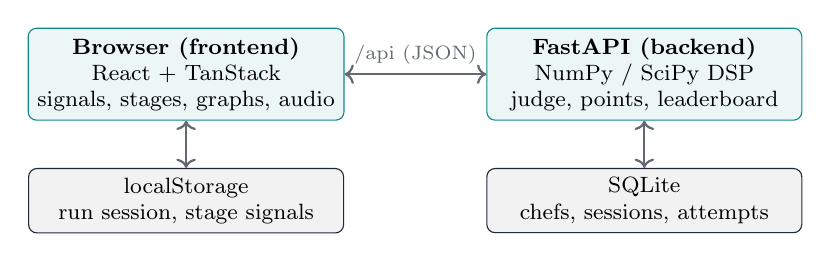
\begin{tikzpicture}[node distance=6mm and 5mm]
\node[st,minimum width=40mm] (fe) {\textbf{Browser (frontend)}\\React + TanStack\\signals, stages, graphs, audio};
\node[st,right=18mm of fe,minimum width=40mm] (be) {\textbf{FastAPI (backend)}\\NumPy / SciPy DSP\\judge, points, leaderboard};
\node[gate,below=of fe,minimum width=40mm] (ls) {localStorage\\run session, stage signals};
\node[gate,below=of be,minimum width=40mm] (db) {SQLite\\chefs, sessions, attempts};
\draw[arr,<->] (fe)--node[above,font=\scriptsize]{/api (JSON)}(be);
\draw[arr,<->] (fe)--(ls); \draw[arr,<->] (be)--(db);
\end{tikzpicture}

\vfill
{\large CSE 220 --- Signals and Linear Systems project}\\[0.2cm]
{\color{wkgrey}Companion to the \emph{Detailed Gameplay Overview}}
\end{titlepage}

\tableofcontents
\newpage

% ====================================================================
\section{System architecture}
% ====================================================================
\subsection{Processes and responsibilities}
\begin{longtable}{@{}P{3.4cm}P{12.1cm}@{}}
\toprule
Part & Responsibility \\
\midrule
\endhead
\file{run.py} & Starts the backend (\texttt{uvicorn app.main:app --reload}, port 8000; on Windows in its own hidden console so its reload Ctrl+C cannot stop the runner) and the Vite dev server (port 5173). Relays backend logs; stops both on exit. \\
Frontend & Synthesises ingredient signals, runs every station's DSP, draws, plays audio, keeps the run in \texttt{localStorage}, and talks to the backend through \file{frontend/src/lib/api.ts} (header \texttt{X-Player-Token}). \\
Backend & Owns chefs (hashed passwords, tokens), sessions and attempts; regenerates ingredients from a seed; rebuilds and scores the dish; computes points, ranks, tier unlocks and leaderboards. \\
\bottomrule
\end{longtable}

\subsection{Frontend storage (\texttt{localStorage})}
\begin{longtable}{@{}P{6.2cm}P{9.3cm}@{}}
\toprule
Key & Contents \\
\midrule
\endhead
\file{wavebakery_recipe_session} & The run: recipe, difficulty, start/end time, every stage accuracy, every dial (seasoning, marinate, appliance, bowl, chop, caramelize, cart), final score/stars, backend session id and result. Type \fn{RecipeRunSession} in \file{lib/recipes.ts}. \\
\file{wavebakery_progress_<recipe>} & Highest unlocked level (1--9). \\
\file{wavebakery_pipeline_<recipe>_<stage>} & A saved \fn{PipelineSignal} for stage \texttt{raw, filtered, mixed, seasoned, marinated, cooked, delivered}. \\
\file{wavebakery_filtered_ingredients_<recipe>} & Filtered samples per washable ingredient. \\
\file{wavebakery_cooked_signal_<recipe>} & The cooked dish (\fn{CookedSignalData}). \\
\file{wavebakery_selected_ingredients_<recipe>} & Ingredients picked in Generate. \\
\file{wavebakery_leaderboard_entries} & The on-device leaderboard. \\
\file{wavekitchen_player_token}, \file{wavebakery_chef_name} & Server token and chef name. \\
\file{wavebakery_recipe_best_scores} & Best total per recipe. \\
\bottomrule
\end{longtable}
Changing a stage calls \fn{invalidateDownstreamStages} (\file{lib/pipeline.ts}), which deletes
every later stage's saved signal so nothing stale is carried forward.

\subsection{Backend tables (\file{backend/app/models.py})}
\begin{longtable}{@{}P{3.4cm}P{12.1cm}@{}}
\toprule
Table & Fields that matter \\
\midrule
\endhead
\texttt{players} & handle, token, scrypt \texttt{password\_hash}, points, unlocked tier. \\
\texttt{ingredients}, \texttt{appliances}, \texttt{recipes} & Catalogue from \file{seed.py}; recipes hold targets (seasoning, blend, marinate, caramelize carrier/depth, chop factor, appliances), tier, tolerance, noise difficulty. \\
\texttt{game\_sessions} & One run: seed, status (\texttt{active/served/abandoned}), difficulty, params (JSON). \\
\file{session_ingredients} & Per-slot seed, contaminants, filter bands/tools, prep score, accepted. \\
\texttt{attempts} & A served dish: score, stars, prep score, SNR, MSE, correlation, spectral similarity, points, difficulty, notes. The leaderboard's source. \\
\bottomrule
\end{longtable}

% ====================================================================
\section{Conventions: how a signal is represented}
% ====================================================================
\subsection{The \texttt{PipelineSignal}}
Every frontend stage produces
\[
\mathbf{x}=\bigl(x[0],\dots,x[N-1]\bigr),\qquad N=401,\qquad t_n=\tfrac{n}{N-1}\in[0,1],
\]
plus metadata (frequency label, duration label, and optionally the 2-D mixing curve).
A frequency of $f$ ``game Hz'' means $f$ cycles in the window.

\begin{mathbox}{Helper functions (\file{frontend/src/lib/pipeline.ts})}
\begin{itemize}[leftmargin=*]
\item \fn{sampleAt}$(\mathbf{x},u)$: periodic linear interpolation. With $u'=u \bmod 1$,
  $p=u'(N-1)$, $i=\lfloor p\rfloor$:
  $\;x(u)=x[i]+(p-i)\,(x[i+1]-x[i])$.
\item \fn{resampleSignal}$(\mathbf{x},M)$: $y[m]=\text{sampleAt}(\mathbf{x},m/(M-1))$.
\item \fn{normalizeSamples}$(\mathbf{x},0.95)$: scales \emph{down only}:
  $y=x\cdot\min(1,\,0.95/\max_n|x[n]|)$.
\end{itemize}
\end{mathbox}

\subsection{From samples to sound (\file{frontend/src/lib/audio.ts})}
\fn{SignalAudioPlayer} treats the window as one period-group and loops it. With the
signal's frequency label $f$ (default 4),
\[
f_0=\operatorname{clip}\!\left(220\cdot\tfrac{f}{4},\,110,\,880\right)\text{ Hz},\qquad
\text{windows per second}=\frac{f_0}{\max(1,f)} .
\]
Output sample $k$ at the device rate $F_s$ ($t=k/F_s$) is
$s(t)=x\bigl((t\cdot f_0/f)\bmod 1\bigr)\cdot g\cdot e(t)$ with gain
$g=0.75/\max|x|$ and a 30\,ms attack / 120\,ms release envelope $e(t)$. So the audible
fundamental is $f_0$ and the timbre is exactly the drawn waveform. The recorded chicken
plays its decoded WAV buffer directly.

\textbf{Loop seam} (\fn{smoothLoopSeam}): looping jumps from $x[N-1]$ back to $x[0]$. If that
jump is larger than $1.5\times$ the largest step inside the signal (a signal that does not
complete whole cycles in the window, e.g.\ carrot, milk or a delayed dish), the last 5\,\% of
the window is blended towards $x[0]$ with a raised-cosine ramp
$x[n]+\bigl(x[0]-x[N-1]\bigr)\tfrac12\bigl(1-\cos\pi u\bigr)$, removing the click that would
otherwise repeat at the loop rate. Genuine edges (square waves) are left untouched.

% ====================================================================
\section{Signal generation}
% ====================================================================
\subsection{Frontend ingredient models (\file{frontend/src/lib/signals.ts})}
Each ingredient is an \fn{IngredientSignalDefinition} with \fn{evaluate},
\fn{generateSamples} and, for 2-D shapes, a \fn{parametricCurve}. The router
\fn{getRecipeIngredientSamples} (\file{lib/pipeline.ts}) returns 401 samples:
\begin{enumerate}
\item \textbf{Chicken} $\rightarrow$ \fn{generateChickenSamples}: linear interpolation of the decoded PCM
  (\file{lib/chicken-samples.ts}) over the whole 2.16\,s clip.
\item \textbf{Catalogued ingredient} $\rightarrow$ its \fn{generateSamples}$(f,A,\phi,\text{noise})$.
\item \textbf{Fallback}: $x[n]=A\sin(2\pi f t_n+\phi)$.
\end{enumerate}

\begin{mathbox}{Periodic families}
\begin{align*}
\text{triangle (Cheese)}:&\quad x(t)=A\tfrac{2}{\pi}\arcsin\bigl(\sin(2\pi ft+\phi)\bigr)
  = \tfrac{8A}{\pi^2}\sum_{k\ \text{odd}}\tfrac{(-1)^{(k-1)/2}}{k^2}\sin(2\pi kft+\dots)\\
\text{square (Sugar, Salt)}:&\quad x(t)=A\,\mathrm{sgn}\bigl(\sin(2\pi ft+\phi)\bigr)
  = \tfrac{4A}{\pi}\sum_{k\ \text{odd}}\tfrac{1}{k}\sin(2\pi kft+\dots)
\end{align*}
The Fourier series explains what the Filtering and Oven spectra show: a square wave keeps
strong odd harmonics ($1/k$), a triangle loses them quickly ($1/k^2$).
\end{mathbox}

\begin{mathbox}{Parametric ingredients and their 1-D signal}
A curve $\gamma(\theta)=(X(\theta),Y(\theta))$, $\theta\in[\theta_{\min},\theta_{\max}]$, is
sampled at 601 points for drawing. The 1-D signal uses the vertical component over the
same parameter range, e.g.\ Noodles ($\theta\in[-12\pi,12\pi]$):
\[
x[n]=A\cos\bigl(-12\pi+24\pi\,t_n+\phi\bigr)\quad(\text{i.e. }Y/5).
\]
\end{mathbox}

\begin{mathbox}{Frontend noise model (\fn{ingredientNoise})}
Five tones above the ingredient's band (15.3, 18.7, 22.1, 26.9, 31.4 game Hz):
\[
n(t)=0.85\,\nu\,\frac{1}{5}\sum_{i=1}^{5}\sin\bigl(2\pi f_i t+37.1\,\phi_s\,i\bigr),
\qquad x_{\text{dirty}}=x-n .
\]
Tones are used instead of a hashed pseudo-random sequence so the noise is genuinely spread
above the cutoff instead of aliasing into one spike.
\end{mathbox}

\subsection{Backend ingredient synthesis and contamination}
Backend signals are real audio: $F_s=22\,050$\,Hz, frame length $4096$ ($\approx186$\,ms)
(\file{backend/app/dsp/core.py}). \fn{clean_signal} calls \fn{instruments.synth} (additive
partials with ADSR envelopes: piano, guitar, bell, flute, \dots, plus mathematical voices for
cheese, sugar, salt, bread, patty, carrot, cucumber, sauce, egg).

\fn{contamination.corrupt}(clean, difficulty $d$, seed) uses a seeded RNG so the same session
always reproduces the same dirty ingredient:
\begin{itemize}
\item number of layers $=1+\text{rand}\{0,\dots,\min(2,\lfloor d\rfloor)\}$;
\item each layer's amplitude $a=0.08+0.10\,d\,(0.6+0.8u)$, $u\sim U(0,1)$;
\item type chosen from \{\textbf{white} (whole band), \textbf{hiss} (high-passed noise starting
  just above the ingredient's ideal cutoff $\times(1.1..1.6)$), \textbf{burst} (sparse clicks)\};
\item $x_{\text{dirty}}=x+\sum_\ell n_\ell$, and every contaminant's band $[f_{lo},f_{hi}]$ is recorded.
\end{itemize}

% ====================================================================
\section{Filtering}
% ====================================================================
\subsection{Server filter (authoritative)}
\fn{apply_filter_chain} (\file{backend/app/dsp/pipeline.py}) is an FFT-mask filter:
\[
N=2^{\lceil\log_2 L\rceil},\quad X[k]=\mathrm{FFT}_N\{x\},\quad
Y[k]=X[k]\,H(f_k),\quad f_k=\tfrac{kF_s}{N},\quad y=\mathrm{IFFT}_N\{Y\}[0..L-1].
\]
The player's cutoff becomes a low-pass tool with a raised-cosine transition of width
$w=\max(30,\,0.15f_c)$ (\fn{core.lowpass}):
\[
H(f)=\begin{cases}1 & f\le f_c\\[2pt]
1-\tfrac12\bigl(1-\cos\pi\tfrac{f-f_c}{w}\bigr) & f_c<f<f_c+w\\[2pt]
0 & f\ge f_c+w\end{cases}
\]
(Graphic-EQ bands, high-pass, band-pass, notch and a harmonic ``de-hum'' comb are built the
same way and multiplied: \fn{chain}.)

\subsection{Cleaning (prep) score --- \fn{metrics.prep_quality}}
With magnitude spectra $C$ (clean), $D$ (dirty), $F$ (filtered) and the set of noise bins
$\mathcal{B}$ (inside any contaminant band):
\begin{align*}
\text{noise}_{\text{before}}&=\sum_{k\in\mathcal B}\max(0,D_k-C_k), &
\text{noise}_{\text{after}}&=\sum_{k\in\mathcal B}\max(0,F_k-C_k),\\
\text{removal}&=\operatorname{clip}\Bigl(1-\tfrac{\text{noise}_{\text{after}}}{\text{noise}_{\text{before}}},0,1\Bigr), &
\text{preservation}&=\operatorname{clip}\Bigl(\tfrac{\sum_k\min(C_k,F_k)}{\sum_k C_k},0,1\Bigr),
\end{align*}
\[
\text{prep}=100\,(0.55\,\text{removal}+0.45\,\text{preservation}).
\]
Flags: \emph{over-filtered} if preservation $<0.55$; \emph{still dirty} if removal $<0.5$.
\fn{accept_ingredient} rejects prep $<45$ or either flag. It is deliberately not a
distance to the clean signal, which would reward doing nothing when the noise is quiet.

\subsection{Frontend Filtering Lab (\file{routes/filtering.tsx})}
\begin{enumerate}
\item Input: the server's dirty/clean plots for the slot when a session exists, otherwise
  \fn{getRecipeIngredientSamples} with noise $0.85$ (dirty) and $0$ (clean).
\item Live preview while dragging (cutoff $f_c\in[0,900]$, ideal $f^\star$):
  noise $=\text{dirty}-\text{clean}$;
  if $f_c<f^\star$: signal gain $\max(0,1-\tfrac{f^\star-f_c}{200})$, noise gain $0$;
  else noise gain $\bigl(\tfrac{f_c-f^\star}{900-f^\star}\bigr)^{1.5}$.
\item \emph{Apply}: sends a low-pass tool with that cutoff to the server and shows its
  filtered plot and prep score. Cleanliness $=$ server prep score (offline: the similarity of
  filtered vs clean, or $97-|f_c-f^\star|/6$ before applying).
\item Pass mark: cleanliness $\ge 85$. \emph{Advance} accepts the ingredient on the server,
  saves the filtered samples (\fn{saveFilteredIngredient}) and records the stage accuracy
  as the running average of cleanliness over the washed ingredients.
\end{enumerate}

% ====================================================================
\section{Mixing}
% ====================================================================
\begin{mathbox}{\fn{computeMixedSignal} (\file{lib/pipeline.ts})}
For bowl ingredients $k=1..K$ with samples $x_k$ (the saved filtered samples if the
ingredient was washed, otherwise its generated samples, noisy if washable):
\[
m[n]=\text{normalize}_{0.95}\Bigl(\tfrac{1}{\sqrt K}\sum_{k=1}^{K}x_k[n]\Bigr),\qquad
K=1:\ m=x_1\ \text{(pass-through)} .
\]
The $1/\sqrt K$ factor keeps the RMS of $K$ uncorrelated signals comparable to one signal.
\end{mathbox}

\begin{mathbox}{The mixing-bowl curve (\fn{computeSuperpositionCurve}, \fn{withMixCurve})}
If any bowl ingredient is parametric, the bowl is the geometric sum at a common
normalised parameter $u\in[0,1]$ (601 points):
\[
X(u)=\sum_{k\in\text{param}}X_k(\theta_k(u)),\qquad
Y(u)=\sum_{k\in\text{param}}Y_k(\theta_k(u))+\sum_{j\in\text{1-D}}x_j(u).
\]
The curve is attached as metadata (\texttt{curve}); the samples $m[n]$ are unchanged, so
filtering still reaches the mix. Later stages transform the curve alongside the samples
(\fn{transformCurve}, \fn{delayCurve}, \fn{carryCurve}) and \fn{pipelineSignalToPath} draws it.
\end{mathbox}

\textbf{Accuracy} (\fn{handleMix}, \file{routes/mixing.tsx}):
$\text{mix}=100\cdot\frac{|\text{bowl}\cap\text{recipe}|}{|\text{recipe}|}$. The bowl's
ingredient names are stored in the session and synced to the server.

\textbf{Server} (\fn{bowl_signals}, \fn{stage_mix}): recipe ingredients in the bowl use their
filtered signal, extra catalogue ingredients are added clean, missing ones are absent; then
$m=\frac{1}{\sqrt K}\sum_k \text{resize}(x_k,4096)$.

% ====================================================================
\section{Seasoning, marinating, caramelizing, chopping}
% ====================================================================
\subsection{Seasoning --- \fn{computeSeasonedSignal}}
\[
s[n]=A\cdot m\bigl((\alpha\,t_n)\bmod 1\bigr)\qquad(\text{via \fn{timeScaleSamples}}),
\]
i.e.\ $y(t)=A\,x(\alpha t)$ with the mix repeated periodically when $\alpha>1$. No
renormalisation, so $A$ really changes the height. The frequency label becomes $\alpha f$.
The curve: $Y\mapsto Y_{\text{mid}}+A(Y-Y_{\text{mid}})$, parameter sped up by $\alpha$ with an
$x$-offset per repeat. \textbf{Accuracy} (\file{routes/transform.tsx}):
\[
\text{acc}=\max\Bigl(0,\,100-70\bigl(\tfrac{|A-A^\star|}{A^\star}+\tfrac{|\alpha-\alpha^\star|}{\alpha^\star}\bigr)\Bigr),
\quad\text{pass at }85.
\]
\textbf{Server}: \fn{stage_season} $y=A x$; \fn{stage_blend} $y[n]=x(\alpha n)$ by linear
interpolation with zeros past the end (\fn{core.time_scale}); length becomes $\lfloor L/\alpha\rceil$.

\subsection{Marinating --- \fn{computeMarinatedSignal}}
With time $s$ (seconds) and duration label $D=3$:
\[
d=\operatorname{round}\!\Bigl(\tfrac{s}{\max(1,D)}\cdot N\Bigr),\qquad
r[n]=\begin{cases}m\bigl(\tfrac{n-d}{N-1}\bigr) & 0\le n-d\\ 0 & n<d\end{cases},
\qquad r\leftarrow\text{normalize}_{0.95}(r).
\]
The curve gets a flat lead-in at the centre line (\fn{delayCurve}).
\textbf{Accuracy}: $\max\bigl(0,\,100-150\tfrac{|s-s^\star|}{s^\star}\bigr)$, pass at 85.
\textbf{Server}: \fn{stage_marinate} delays by $sF_s$ samples after zero-padding; integer
delays copy samples, fractional delays use the shift theorem
\[
Y[k]=X[k]\,e^{-j2\pi k\,d/N}\qquad(\fn{core.time_shift}).
\]

\subsection{Caramelizing --- amplitude modulation}
Frontend (\file{routes/caramelize.tsx}): $y[n]=r[n]\bigl(1+m\cos(2\pi\tfrac{f_c}{10}t_n)\bigr)$,
then normalised to $0.95$; \textbf{accuracy}
$=\operatorname{clip}\bigl(100-45\tfrac{|f_c-180|}{180}-55|m-0.55|,\,10,\,100\bigr)$.
Server (\fn{core.am_modulate}): $y(t)=x(t)\,[1+m\cos(2\pi f_c t)]$ with $t$ in seconds.
In frequency: $Y(f)=X(f)+\tfrac m2X(f-f_c)+\tfrac m2X(f+f_c)$ --- two sidebands.

\subsection{Chopping --- decimation}
Frontend (\file{routes/chop.tsx}): zero-order-hold decimation by $M$,
$y[n]=x\bigl[M\lfloor n/M\rfloor\bigr]$; the effective rate is $22050/M$ and ``aliasing''
is declared when anti-aliasing is off, $M>1$ and $800f>22050/(2M)$, in which case a
synthetic tone of $|22050/M-800f|/100$ cycles per window and amplitude 0.35 is added (a simulation, not true folding). \textbf{Accuracy}:
$\max(20,\,100-25|M-3|)$, minus 35 (floor 15) without anti-aliasing.
Server (\fn{core.decimate}): optional low-pass at $0.9\cdot\tfrac{F_s}{2M}$, keep every $M$-th
sample, zero-order hold back to the original length; new Nyquist $F_s/(2M)$.

% ====================================================================
\section{Cooking --- convolution}
% ====================================================================
\subsection{Impulse responses}
Frontend kernels (\fn{generateStaticCookingKernel}, 96 taps, $\sum_k|h[k]|=1$):
\begin{align*}
h_{\text{grill}}[k]&=e^{-k/16}\bigl(\tau_k+0.15\sin(1.85k)e^{-k/16}\bigr),\ \ \tau_k\ \text{taps }1,.55,.38,.22,.12,.06\text{ at }k=0,4,11,21,35,54\\
h_{\text{fry}}[k]&=e^{-k/22}\bigl(0.45\sin(12.99k+3.14)+0.35\sin(31.42k+1.2)+0.2\cos(57.17k)\bigr)\\
h_{\text{bake}}[k]&=e^{-((k-16)/14)^2}\quad\text{(Gaussian, a smooth low-pass)}\\
h_{\text{boil}}[k]&=e^{-k/26}\bigl(0.7\sin(\pi k/7)+0.3\sin(\pi k/14)\bigr)\quad\text{(damped resonator)}
\end{align*}
Server impulse responses (\file{backend/app/dsp/systems.py}): grill = comb (delay 90, feedback
0.62, 7 taps), fry = short bright decay ($\tau=130$), bake = long dark decay ($\tau=700$,
low-passed), boil = resonator $e^{-k/\tau}\sin(2\pi f_0k/F_s)$ at 320\,Hz, simmer = 48-tap moving
average, sear $=[1,-1]$ (differencer), plus smoke and steam composites.

\subsection{\fn{computeConvolvedSignal} (\file{lib/pipeline.ts})}
Slider position $p\in[0,100]$, $\tau=p/100$, shift $s=\operatorname{round}(30\tau)$:
\[
c[n]=\sum_{k=0}^{95}x\bigl((n-k-s)\bmod N\bigr)\,h[k]\quad\text{(circular convolution)},
\]
\[
y[n]=(1-w)\,x[n]+w\,c[n],\qquad w=\min(1,1.15\tau),
\]
plus a small crackle $0.04\tau\sin(27.13n+7.4)$ for frying, then normalised to $0.95$.
\textbf{Accuracy} (\file{routes/cooking.tsx}): $50$ if the recipe's method is chosen (else 15)
$+\min(50,\,p/2)$. The target cooked signal uses the recipe's method at $p=100$.

\textbf{Server} (\fn{stage_cook}, \fn{apply_system}): linear convolution $y=x*h$ (SciPy,
direct or FFT), truncated to the input length, rescaled to $0.95$ only if it clips.
Several appliances are one system: \fn{cascade} $h=h_1*h_2*\cdots$.

% ====================================================================
\section{Precision Oven (\file{frontend/src/lib/precision-oven-dsp.ts})}
% ====================================================================
\subsection{Maximum frequency and the Nyquist rate}
\fn{findMaxSignalFrequency}: resample the dish to 128 points, apply a Hann window
$w[n]=\tfrac12(1-\cos\frac{2\pi n}{127})$, FFT, and take the first bin $k$ at which the
cumulative energy $\sum_{i=1}^{k}|X_i|^2$ reaches 95\,\% of the total (DC excluded);
with a 128-point window over one second each bin is 1 game Hz wide, so $f_{\max}=\operatorname{clip}(k,2,32)$ game Hz. Minimum safe
rate $=2f_{\max}$.

\subsection{Sampling and aliasing demonstration --- \fn{analyzeSamplingAndAliasing}}
\begin{enumerate}
\item Samples $x_m=x(m/f_s)$ for $m=0..\lfloor f_s\rceil-1$ over the one-second window.
\item Periodic sinc reconstruction over three periods:
  $\hat x(t)=\sum_{p=-1}^{1}\sum_m x_m\,\mathrm{sinc}\bigl(f_s(t-\tfrac{m}{f_s}-p)\bigr)$.
\item Folding of the five strongest harmonics when $f>f_s/2$:
  $f_{\text{alias}}=|f-\operatorname{round}(f/f_s)f_s|$ (reflected again if still above $f_s/2$).
\end{enumerate}

\subsection{Spectrum used for tuning --- \fn{computeDiscreteSignalFFT}}
\[
N_{\text{FFT}}=\max(64,\,2^{\lceil\log_2 f_s\rceil}),\quad
x[m]=x(m/f_s)\ (m<f_s),\ \ 0\ \text{otherwise (zero padding)},\quad
f_k=\frac{k\,f_s}{N_{\text{FFT}}}.
\]
No window is applied (the edited spectrum is inverted back). Displayed magnitude
$|X_k|\cdot 2/f_s$, normalised by $1.25\max$. Radix-2 Cooley--Tukey FFT with bit reversal
(\fn{cooleyTukeyRadix2}). Bins are classed as Base Warmth $[0,6)$, Crumb $[6,16)$, Top Crisp
$[16,32]$ game Hz (\fn{getBandAvailability} marks a band unavailable/partial when
$f_s/2$ is below it).

\subsection{Equaliser --- \fn{tuneOvenFrequencies}}
\[
X'_k=X_k\cdot G_{\text{band}(f_k)}\cdot C(f_k)\cdot Q(f_k),\qquad
C(f)=\begin{cases}1&f\le f_c\\ \max\!\bigl(0.01,e^{-((f-f_c)/4)^2}\bigr)&f>f_c\end{cases},
\]
\[
Q(f)=1-\frac{0.88}{1+\bigl((f-f_n)/1.5\bigr)^2}\quad\text{for }|f-f_n|\le3\ (\text{notch on}),
\]
\[
X'_{N-k}=\overline{X'_k}\qquad(\text{Hermitian symmetry, so the result stays real}).
\]

\subsection{Reconstruction --- \fn{computeSignalIFFT}}
IFFT, keep the first $N_s=\lfloor f_s\rceil$ samples, then band-limited periodic interpolation
with the Dirichlet kernel back to 401 points:
\[
\hat x(t)=\sum_{m=0}^{N_s-1}x'_m\,D_{N_s}\!\Bigl(t-\frac{m}{N_s}\Bigr),\qquad
D_N(\tau)=\begin{cases}\dfrac{\sin(\pi N\tau)}{N\sin(\pi\tau)} & N\ \text{odd}\\[8pt]
\dfrac{\sin(\pi N\tau)}{N\tan(\pi\tau)} & N\ \text{even}\end{cases}
\]
then normalised to $0.95$. With untouched controls and $f_s\ge2f_{\max}$ this reproduces the
dish (verified $\ge98\,\%$ similarity by \file{frontend/tests/precision-oven-fft.test.ts}).

\subsection{Oven score}
\begin{align*}
\text{spectrum match}&=\operatorname{clip}\Bigl(100\bigl(1-\tfrac{\sum_k|c_k-t_k|}{1.5\sum_k t_k}\bigr),0,100\Bigr)\ \ (\fn{computeSpectrumSimilarity})\\
\text{waveform fidelity}&=\fn{computeSignalSimilarity}(\hat x,\ \text{target})\ \ (\text{Section~\ref{sec:similarity}})\\
\text{efficiency}&=\begin{cases}100 & f_s\le1.25\cdot2f_{\max}\\
100\bigl(1-\frac{f_s-2.5f_{\max}}{64-2.5f_{\max}}\bigr)^+ & \text{otherwise}\end{cases}\\
\text{oven}&=0.40\,\text{spectrum}+0.50\,\text{fidelity}+0.10\,\text{efficiency}.
\end{align*}
The unlock step rejects $f_s<2f_{\max}$ and $f_s>64$. \emph{Plate} saves the reconstruction as
the \texttt{delivered} stage and records the oven score as the delivery accuracy.

% ====================================================================
\section{System Delivery --- the z-plane (\file{frontend/src/lib/z-system.ts})}
% ====================================================================
\begin{longtable}{@{}P{2.6cm}P{5.6cm}P{7.3cm}@{}}
\toprule
Preset & $H(z)$ & Poles / zeros / gain \\
\midrule
\endhead
1st-order low-pass & $\dfrac{(1-r)z}{z-r}$;\ $y[n]=(1-r)x[n]+ry[n-1]$ & pole $r$, zero $0$, $g=1-r$ (unity DC gain) \\
2nd-order resonator & $\dfrac{z^2}{(z-re^{j\omega_0})(z-re^{-j\omega_0})}$ & conjugate poles, double zero at 0, $g=1$; $y[n]=x[n]+2r\cos\omega_0\,y[n-1]-r^2y[n-2]$ \\
Moving average & $\tfrac16\dfrac{1-z^{-6}}{1-z^{-1}}$ & zeros $e^{j2\pi k/6}$, $k=1..5$; five poles at 0; $g=1/6$ (FIR) \\
Notch & $\dfrac{(z-e^{j\omega_0})(z-e^{-j\omega_0})}{(z-0.85e^{j\omega_0})(z-0.85e^{-j\omega_0})}$ & zeros on the unit circle, poles at radius 0.85 \\
\bottomrule
\end{longtable}

\begin{mathbox}{Frequency response and filtering}
\begin{itemize}[leftmargin=*]
\item Magnitude on the unit circle, geometrically (\file{SystemResponsePlotter.tsx}):
  $|H(e^{j\omega})|=g\,\frac{\prod_i|e^{j\omega}-z_i|}{\prod_j|e^{j\omega}-p_j|}$ (clipped to 4),
  phase $=\sum\arg(e^{j\omega}-z_i)-\sum\arg(e^{j\omega}-p_j)$, 128 points on $[0,\pi]$.
\item Dish spectrum: 64-point DFT of the dish; bin $k\le32$ sits at $\omega_k=2\pi k/64$ and is
  multiplied by $|H(e^{j\omega_k})|$ (an unstable cart shows $\times5$).
\item Actual filtering (\fn{applySystem}): expand $\prod(z-p_j)$ and $g\prod(z-z_i)$ into real
  coefficients $a$, $b$ (\fn{expandRoots}), then run the difference equation
  $y[n]=\sum_k b_kx[n-k]-\sum_{k\ge1}a_ky[n-k]$. This plays as ``Listen equalized dish''.
\end{itemize}
\end{mathbox}

\textbf{Score} (\fn{systemAccuracy}; server \fn{system_score_for} computes the same from the
synced settings): $100$ if $\max_j|p_j|<1$ (BIBO stable) else $15$, multiplied by $0.6$ when
the sensor rate is below $4000$\,Hz.

% ====================================================================
\section{Similarity metrics}\label{sec:similarity}
% ====================================================================
\subsection{Frontend (\fn{computeSignalSimilarity}, \file{frontend/src/lib/dsp.ts})}
The player's samples are resampled to the target length, then
\[
r_{xy}=\frac{\sum(x-\bar x)(y-\bar y)}{\sqrt{\sum(x-\bar x)^2\sum(y-\bar y)^2}},\qquad
\text{NRMSE}_{\text{sim}}=\operatorname{clip}\Bigl(1-\frac{\sqrt{\tfrac1N\sum(x-y)^2}}{\max y-\min y},0,1\Bigr),
\]
\[
\text{similarity}=100\bigl(0.5\max(0,r_{xy})+0.5\,\text{NRMSE}_{\text{sim}}\bigr).
\]
Correlation rewards the right \emph{shape}; NRMSE rewards the right \emph{level}.

\subsection{Server dish score (\fn{metrics.dish_metrics})}
Both dishes are normalised to peak $0.9$; then
\begin{align*}
\text{SNR}&=10\log_{10}\frac{\sum t^2}{\sum(t-p)^2}\ \text{dB}, &
\text{corr}&=\max_\ell\frac{(t\star p)[\ell]}{\|t\|\,\|p\|}\ \ (\text{peak of the cross-correlation}),\\
\text{spec}&=\frac{\langle T_{\text{dB}},P_{\text{dB}}\rangle}{\|T_{\text{dB}}\|\,\|P_{\text{dB}}\|}, &
T_{\text{dB}}&=\max\bigl(20\log_{10}|T|,-80\bigr)+80,
\end{align*}
\[
\text{dish}=100\Bigl(0.40\operatorname{clip}\tfrac{\text{spec}-0.75}{0.25}+0.35\operatorname{clip}(\text{corr})
+0.25\operatorname{clip}\tfrac{\text{SNR}+5}{30}\Bigr)\quad(\text{each clip to }[0,1]).
\]

% ====================================================================
\section{Scoring, step by step}\label{sec:scoring}
% ====================================================================
\subsection{During the run: stage accuracies}
Each station calls \fn{recordStageAccuracy} (\file{lib/recipes.ts}), which clamps to $[0,100]$
and stores it on the run session: filtering, mixing, seasoning, marinating, cooking,
chop, caramelize, delivery (oven), system (cart). Dials are stored too and pushed to the
server by \fn{syncSessionParamsToBackend}. The payload fields are
\fn{seasoning}, \fn{frequency}, \fn{blend}, \fn{marinate}, \fn{appliances}, \fn{bowl},
\fn{carrier}, \fn{depth}, \fn{chop_factor}, \fn{anti_alias}, \fn{delivery_accuracy},
\fn{system_preset}, \fn{system_pole_radius} and \fn{system_sampling_hz}.

\subsection{The reference dish}
\textbf{Frontend} \fn{getIdealDishSignal}: clean mix of all recipe ingredients
(\fn{computeCleanMixedSignal}) $\rightarrow$ seasoning with $(A^\star,\alpha^\star)$ $\rightarrow$
marinating with $s^\star$ $\rightarrow$ convolution with the recipe method at $p=100$.
\textbf{Server} \fn{judge}: \fn{run_pipeline}(clean ingredient signals,
\fn{reference_params}(recipe)) --- the same function that builds the player's dish.

\subsection{Server judgement --- \fn{gameplay.judge}}
\begin{enumerate}
\item Rebuild the player's dish: regenerate each ingredient from its seed, apply the stored
  filters, keep only the bowl, run \fn{run_pipeline} with the stored params:
  mix $\rightarrow$ season ($A$) $\rightarrow$ blend ($\alpha$) $\rightarrow$ marinate ($s$) $\rightarrow$
  caramelize ($f_c,m$) $\rightarrow$ chop ($M$) $\rightarrow$ cook (appliances) $\rightarrow$ normalise $0.9$.
\item $m=$ \fn{dish_metrics}(reference final, player final).
\item Prep average $\bar P$ over washable/contaminated ingredients (all ingredients if none).
\item Sub-scores: filtering $=\bar P$; mixing $=$ dish score of the two mixes; transformation
  $=$ dish score of the two marinated signals; cooking $=$ dish score of
  (player's pre-cooking signal through the recipe's appliances) vs (through the player's).
\item $\text{raw}=0.72\,m_{\text{score}}+0.28\,\bar P$.
\item Finishing stations, when present: $\text{raw}\leftarrow\text{raw}\,(1-W)+\sum w_i v_i$ with
  $(v,w)=(\text{oven},0.10)$ and $(\text{cart},0.05)$, $W=\sum w_i$.
\item Tolerance curve: $\text{score}=100\,(\text{raw}/100)^{\gamma}$,
  $\gamma=1/\max(0.3,\text{tolerance})$ (tolerance $0.75$ for the Feast up to $1.25$ for Toast:
  harder recipes are graded more strictly).
\item Stars: $\ge92\to5$, $\ge80\to4$, $\ge66\to3$, $\ge50\to2$, $\ge32\to1$, else 0.
\item Notes (\fn{_diagnose}): named mistakes from the parameter errors (over/under-seasoned,
  blended, marinated; wrong AM carrier or depth; wrong chop factor; aliasing; wrong appliance
  chain; over-filtered or still-dirty ingredients).
\end{enumerate}

\subsection{Submission (exactly once)}
\fn{submitRunToBackend} (\file{lib/recipes.ts}) syncs the params, then \texttt{POST
/sessions/\{id\}/submit}; concurrent callers share one in-flight request. The server claims the
session atomically (\texttt{UPDATE \dots\ WHERE status != 'served'}); a second submit gets 409; if
judging fails the claim is released. A served session can no longer be edited.

\subsection{What the score screen shows (\file{routes/score.tsx})}
The player dish is the delivered dish if the oven was used, otherwise the cooked dish. The
stage average is the mean of filtering, mixing, seasoning, marinating and cooking, plus chop
and caramelize for recipes that include those stations.
\begin{align*}
\text{similarity}&=\text{computeSignalSimilarity}(\text{player dish},\ \text{reference dish})\\
\text{local}&=0.5\,\text{similarity}+0.5\,\text{stageAvg}\quad(\text{then the finishing-station blend})\\
\text{score}_{100}&=\text{server score if available, otherwise local}\\
\text{base}&=\operatorname{round}(10\cdot\text{score}_{100}\cdot\mu_{\text{diff}}),\qquad
\mu\in\{0.8,1.0,1.25,1.5\}\\
\text{time bonus}&=\operatorname{round}\bigl(\min(2\cdot\text{seconds left},300)\cdot\mu_{\text{diff}}\bigr)\\
\text{total}&=\text{base}+\text{time bonus}.
\end{align*}
A stage with no recorded accuracy counts as 0 (except filtering on a recipe with nothing to
wash, which counts 100). Stars use the server's stars or the same thresholds on
$\text{score}_{100}$. The total, stars and similarity are stored on the session; the
Complete page (\file{routes/complete.tsx}) only displays them.

% ====================================================================
\section{Points, ranks, tiers and leaderboards}
% ====================================================================
\subsection{Career points and ranks (\file{backend/app/gameplay.py})}
\begin{itemize}
\item \fn{award}: if the new score beats the chef's best on that recipe,
  $\text{points}=\operatorname{round}(\text{score}\times\text{tier}\times1.5)$ is added; otherwise 0.
  Runs on a tier the chef has not unlocked earn 0 and do not count for unlocking.
\item \fn{rank_for}: Dishwasher (0), Prep Cook (250), Line Cook (600), Sous Chef (1100),
  Head Chef (1800), Signal Master (2600).
\item \fn{maybe_unlock}: when the chef has cleared $\min(2,\#\text{recipes})$ distinct recipes of
  their current tier with score $\ge60$, the next tier opens.
\end{itemize}

\subsection{Server leaderboards (\file{backend/app/routers/leaderboard.py})}
\begin{description}[style=nextline,leftmargin=0.6cm]
\item[\texttt{GET /leaderboard?recipe\_id=\&difficulty=\&limit=}] All attempts ordered by
  score (then time), de-duplicated to each chef's best, then cut to \texttt{limit}. With a
  difficulty, attempts of that difficulty plus older attempts that have none recorded.
\item[\texttt{GET /leaderboard/global}] Chefs ordered by career points, then best score; with
  rank title and dishes served.
\item[\texttt{GET /stats}] Players, sessions started, dishes served, average score, and per recipe:
  plays, average, best and five-star rate.
\end{description}

\subsection{On-device leaderboard (\file{frontend/src/lib/leaderboard.ts})}
The score screen calls \fn{addLeaderboardEntry} with id
\texttt{run-<recipe>-<difficulty>-<start>}: one entry per chef, recipe and difficulty, keeping
the higher score. \fn{getLeaderboard} filters by recipe and difficulty and sorts by score. The
leaderboard page shows the server's rows when it has any, otherwise these; it also re-submits
a finished run that never reached the server (backend offline) and shows a retry notice.

% ====================================================================
\section{Security and validation}
% ====================================================================
\begin{itemize}
\item Passwords: scrypt ($N=2^{14},r=8,p=1$, 16-byte salt), constant-time comparison
  (\file{backend/app/security.py}). A chef created before passwords existed gets one on first
  sign-in.
\item Every session endpoint checks the token owns the session (\fn{owned_session}).
\item DSP endpoints bound every input (sample rate 1--96\,kHz, $\le200\,000$ finite samples,
  $\le4096$-tap custom impulse, 1--64 speakers).
\item The SPA file route only serves files inside \texttt{frontend/dist}; CORS allows only the
  frontend's origins.
\item The server never trusts client audio: it regenerates ingredients from the seed and
  rebuilds the dish. The one client-reported number is the Precision Oven score.
\end{itemize}

% ====================================================================
\section{Function index}
% ====================================================================
{\small
\begin{longtable}{@{}P{5.6cm}P{3.9cm}P{6.0cm}@{}}
\toprule
Function & File & Mathematical role \\
\midrule
\endhead
\multicolumn{3}{@{}l}{\textbf{Frontend}}\\
\fn{evaluate*Wave}, \fn{generate*Samples} & \file{lib/signals.ts} & Ingredient signal models \\
\fn{ingredientNoise} & \file{lib/signals.ts} & Additive multi-tone noise \\
\fn{computeSuperpositionCurve} & \file{lib/signals.ts} & 2-D geometric superposition \\
\fn{getRecipeIngredientSamples} & \file{lib/pipeline.ts} & Ingredient $\rightarrow$ 401 samples \\
\fn{sampleAt}, \fn{resampleSignal}, \fn{normalizeSamples} & \file{lib/pipeline.ts} & Interpolation, resampling, peak limiting \\
\fn{computeMixedSignal} & \file{lib/pipeline.ts} & Superposition with $1/\sqrt K$ \\
\fn{withMixCurve} & \file{lib/pipeline.ts} & Attach bowl curve \\
\fn{computeSeasonedSignal}, \fn{timeScaleSamples} & \file{lib/pipeline.ts} & $A\,x(\alpha t)$ \\
\fn{computeMarinatedSignal}, \fn{delayCurve} & \file{lib/pipeline.ts} & $x(t-t_0)$ \\
\fn{computeConvolvedSignal} & \file{lib/pipeline.ts} & Circular convolution, wet/dry \\
\fn{carryCurve}, \fn{transformCurve}, \fn{pipelineSignalToPath} & \file{lib/pipeline.ts} & Curve follows each stage (display) \\
\fn{getIdealDishSignal}, \fn{computeCleanMixedSignal} & \file{lib/pipeline.ts} & Reference dish \\
\fn{generateStaticCookingKernel} & \file{lib/cooking-audio.ts} & Impulse responses $h[n]$ \\
\fn{fft}, \fn{applyLowPassFilter}, \fn{convolve} & \file{lib/dsp.ts} & FFT, filtering, convolution \\
\fn{normalizedCrossCorrelation}, \fn{normalizedRootMeanSquareError}, \fn{computeSignalSimilarity} & \file{lib/dsp.ts} & Similarity \\
\fn{findMaxSignalFrequency} & \file{lib/precision-oven-dsp.ts} & 95\,\%-energy bandwidth \\
\fn{analyzeSamplingAndAliasing} & \file{lib/precision-oven-dsp.ts} & Sampling, sinc reconstruction, folding \\
\fn{computeDiscreteSignalFFT}, \fn{cooleyTukeyRadix2} & \file{lib/precision-oven-dsp.ts} & Zero-padded DFT / FFT \\
\fn{tuneOvenFrequencies} & \file{lib/precision-oven-dsp.ts} & Band gains, cutoff, notch \\
\fn{computeSignalIFFT} & \file{lib/precision-oven-dsp.ts} & IFFT + Dirichlet reconstruction \\
\fn{computeSpectrumSimilarity} & \file{lib/precision-oven-dsp.ts} & Spectral match \\
\fn{systemPolesZeros}, \fn{applySystem}, \fn{systemAccuracy} & \file{lib/z-system.ts} & $H(z)$, difference equation, stability \\
\fn{SignalAudioPlayer} & \file{lib/audio.ts} & Sonification \\
\fn{recordStageAccuracy}, \fn{syncSessionParamsToBackend}, \fn{submitRunToBackend} & \file{lib/recipes.ts} & Accuracies, sync, submission \\
\fn{addLeaderboardEntry}, \fn{getLeaderboard} & \file{lib/leaderboard.ts} & Local leaderboard \\
\midrule
\multicolumn{3}{@{}l}{\textbf{Backend}}\\
\fn{fft}, \fn{ifft}, \fn{cooley_tukey_fft} & \file{dsp/core.py} & Transforms \\
\fn{lowpass}, \fn{highpass}, \fn{bandpass}, \fn{notch}, \fn{equalizer}, \fn{chain} & \file{dsp/core.py} & Frequency responses \\
\fn{build_mask}, \fn{apply_mask}, \fn{filter_signal} & \file{dsp/core.py} & FFT-mask filtering \\
\fn{time_scale}, \fn{time_shift} & \file{dsp/core.py} & $x(\alpha t)$, $x(t-t_0)$ \\
\fn{convolve}, \fn{apply_system}, \fn{cascade}, \fn{frequency_response} & \file{dsp/core.py} & LTI systems \\
\fn{am_modulate}, \fn{decimate} & \file{dsp/core.py} & AM, down-sampling \\
\fn{corrupt} & \file{dsp/contamination.py} & Seeded noise \\
\fn{synth} & \file{dsp/instruments.py} & Ingredient audio \\
\fn{ir_comb}, \fn{ir_decay}, \fn{ir_resonator}, \fn{ir_moving_average}, \fn{ir_difference} & \file{dsp/systems.py} & Appliance $h[n]$ \\
\fn{run_pipeline}, \fn{reference_params}, \fn{apply_filter_chain} & \file{dsp/pipeline.py} & The canonical dish pipeline \\
\fn{prep_quality}, \fn{dish_metrics}, \fn{snr_db}, \fn{spectral_similarity}, \fn{stars} & \file{dsp/metrics.py} & Scores \\
\fn{bowl_signals}, \fn{compute_stages}, \fn{judge}, \fn{award}, \fn{maybe_unlock}, \fn{system_score_for} & \file{gameplay.py} & Judging and progression \\
\bottomrule
\end{longtable}}

\end{document}
